% !TEX root = ../main.tex
% !TEX spellcheck = en_GB

\chapter{Results}
\label{chap:results}
This chapter compares the created models with the measurements.

Figures~\ref{fig:allcompareseethrough} and \ref{fig:allcomparewooden} shows the comparisons of the drive unit model, cabinet model and the measurements of the see-through and wooden speakers.
The first striking observation is that generally the models have a lower amplitude than the measured data.
Secondly the models are very linear after the cut-off frequency, whereas the measurements seems to contain some overtones.
A clear similarity in behaviour of the Cabinet Model and the measurements is in the slope, especially when looking at the wooden comparison \cref{fig:allcomparewooden} it is clear that the slope of the Drive Unit Model is not as steep as the measurement, whereas the slope of the Cabinet Model matches the measurement very well.
Both the speaker measurements and their models exhibit matching cut-off frequencies.

\begin{figure}
	\centering
	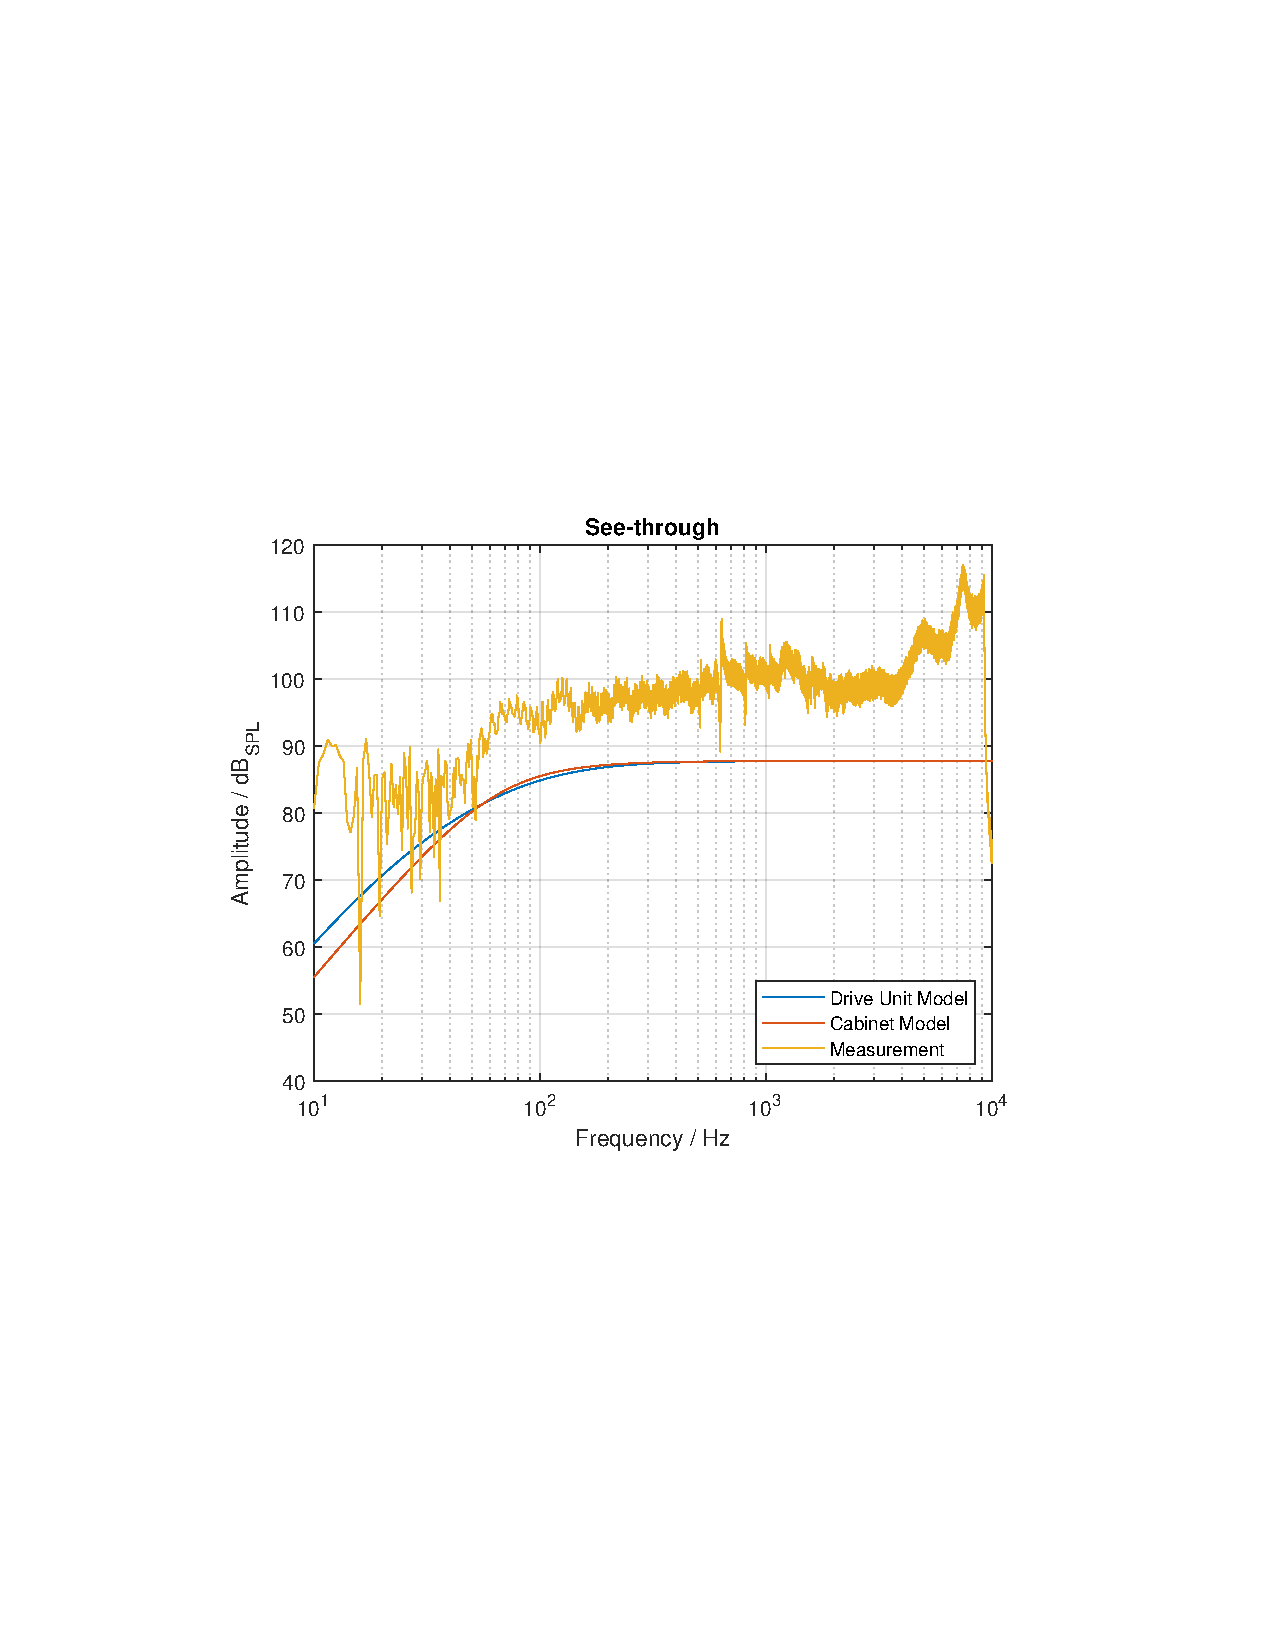
\includegraphics[width=0.7\linewidth, clip, trim={3.9cm 8.4cm 4.5cm 8.5cm}]{gfx/Results/AllCompareSeeThrough.pdf}
	\caption{The two models for the Drive Unit (blue), Cabinet (red) and the measurement of the see-through speaker (orange).}
	\label{fig:allcompareseethrough}
\end{figure}

\begin{figure}
	\centering
	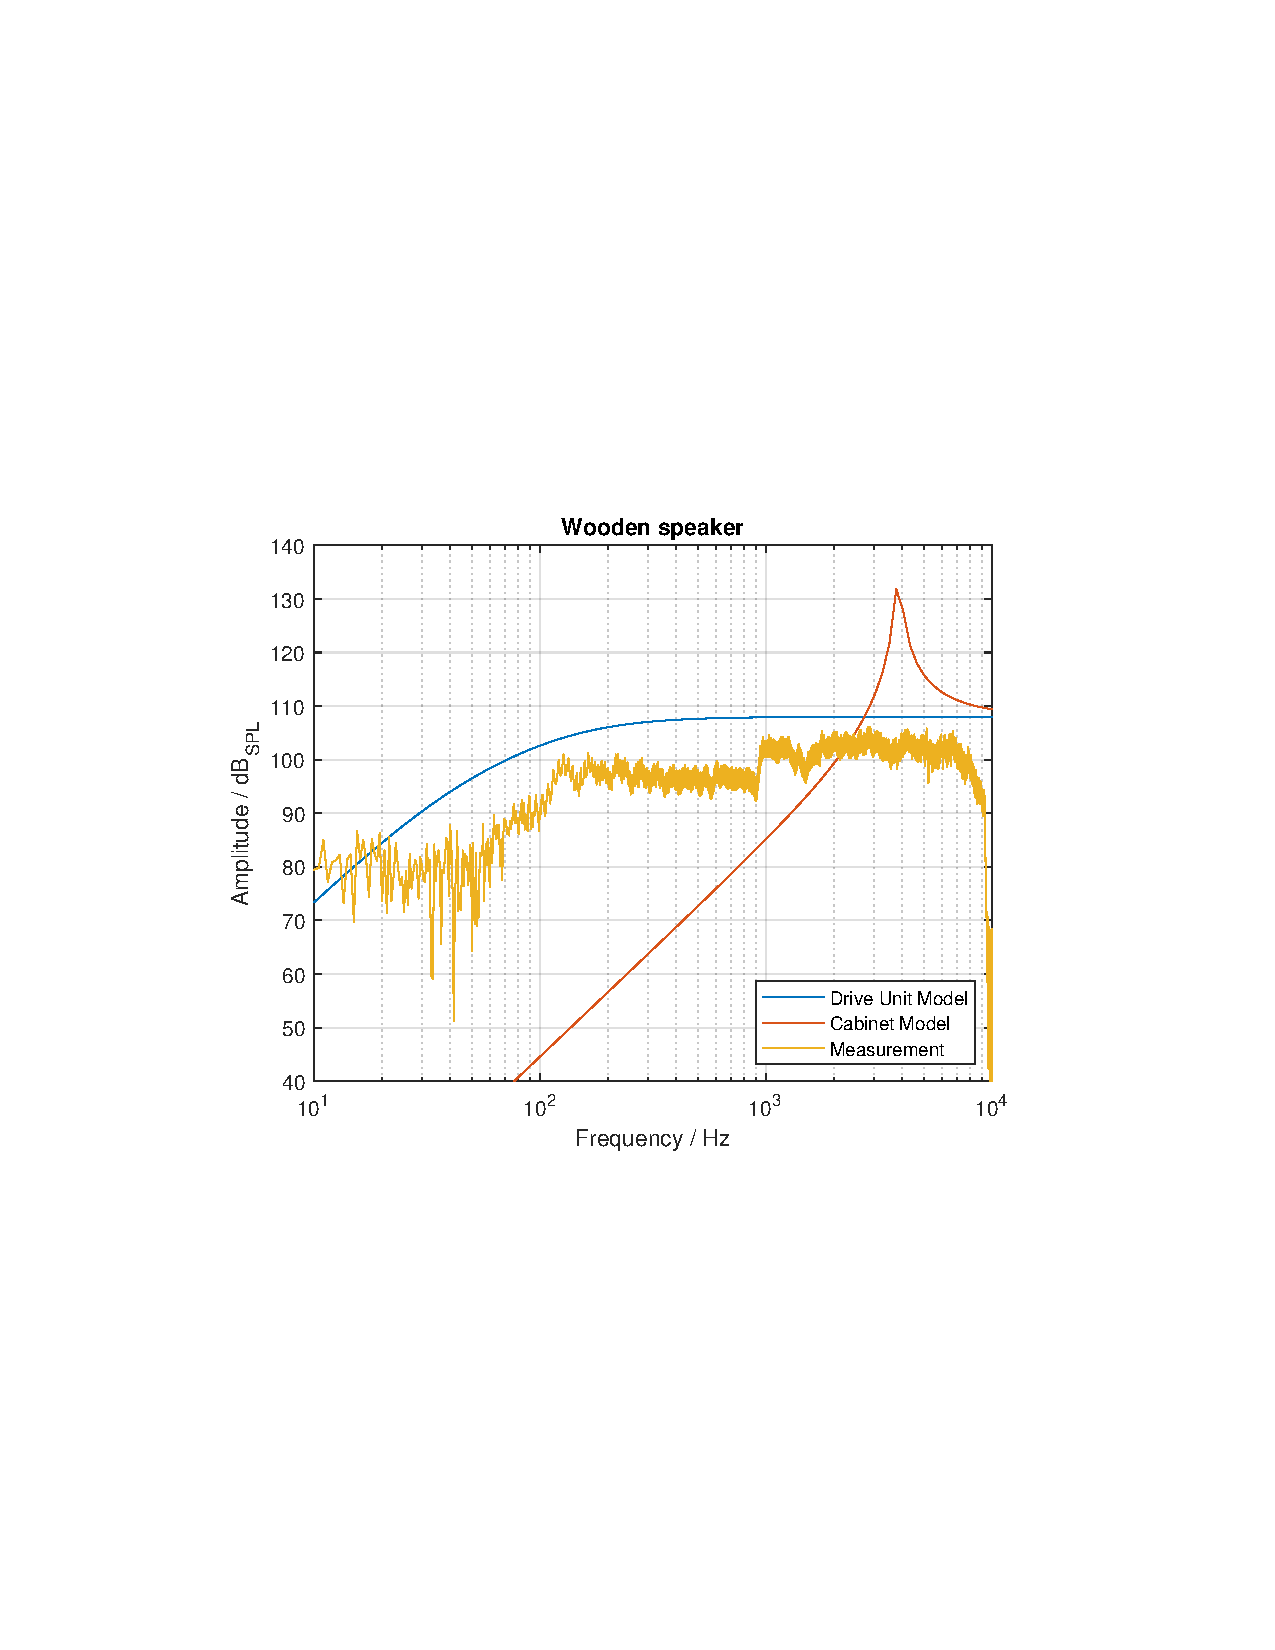
\includegraphics[width=0.7\linewidth, clip, trim={3.9cm 8.4cm 4.5cm 8.5cm}]{gfx/Results/AllCompareWooden.pdf}
	\caption{The two models for the Drive Unit (blue), Cabinet (red) and the measurement of the wooden speaker (orange).}
	\label{fig:allcomparewooden}
\end{figure}

\fxnote{Compare: DUmodel(ST, wood) with meas(ST, wood). Show CABmodel and say not alike.}
\fxnote{Compare \cref{fig:PGcompareAll} with expected effect of bass reflex}
\fxnote{Resonance freq. p. 55 TAS}
\FloatBarrier